%!TEX root = ../TTK4900-MHT.tex
%!TEX root = ../TTK4900-MHT.tex

\chapter{Results}\label{chapter:results}
\section{Testing scheme}
The performance evaluation of the MHT tracking system is tedious in that it is necessary to test very many different situations to get a good understanding of how the system is performing. The two largest factors contributing to the difficulty is the random nature of the clutter and lost detections. It is also desirable to evaluate the initialization and tracking performance under both varying environmental (external) conditions and tuning (internal) setting. We want good tracking of targets with low probability of detections in cluttered environment, and secondly it must be able to do this within the time frame of the radar rotation period. The initialization module must be able to detect targets with probability of detection lower than unity without initializing too may false tracks into the MHT algorithm.

The testing is separated into two parts; initialization and tracking. The performance metrics for the initialization module is how long time it takes to initialize the correct tracks, which is tested under a range of internal and external conditions, see (\ref{eq:init_test_table}). All combinations of these parameters were simulated on all four scenarios from~\ref{sec:scenario}, which are the same routes but with different \gls{ais} configurations. From these simulations, the time to initiate true targets and amount of false targets are calculated and plotted.
\begin{equation}{H}\label{eq:init_test_table}
\begin{split}
\V{P_D} &= \begin{bmatrix} 1.0 & 0.8 & 0.6 \end{bmatrix} \\
\V{M/N} &= \begin{bmatrix} 	(1/1) & (1/2) & (1/3) & (1/4) \\
							(2/2) & (2/3) & (2/4) & (2/5) \\
							(3/3) & (3/4) & (3/5) & (3/6)
		   \end{bmatrix} \\
\V{\lambda_\phi} &= \begin{bmatrix} 0 & 2\cdot10^{-6} & 4\cdot10^{-6} \end{bmatrix}
\end{split}
\end{equation}

When testing the tracking performance, it is desirable to remove the variable of initialization. Therefore are all the simulations testing the tracking performance carried out with all targets correctly initialized at start time, and with the initiator set to \(M=2, N=4\).


\section{Scenario}\label{sec:scenario}
All simulations in this work is based on a generated scenario, as shown in Figure~\ref{fig:test_scenario} with black dots marking the initial time and position. The radar range is 5500 meter (~3 \glspl{nm_acr}), which gives an area of surveillance of approximately 95 square km. The scenario contains 16 targets, which all starts inside the observable area of the radar. The scenario contains a mixture of fast and slow moving vessels, some with sharp turns and some almost at stand still. 
\begin{figure}[H]
\centering
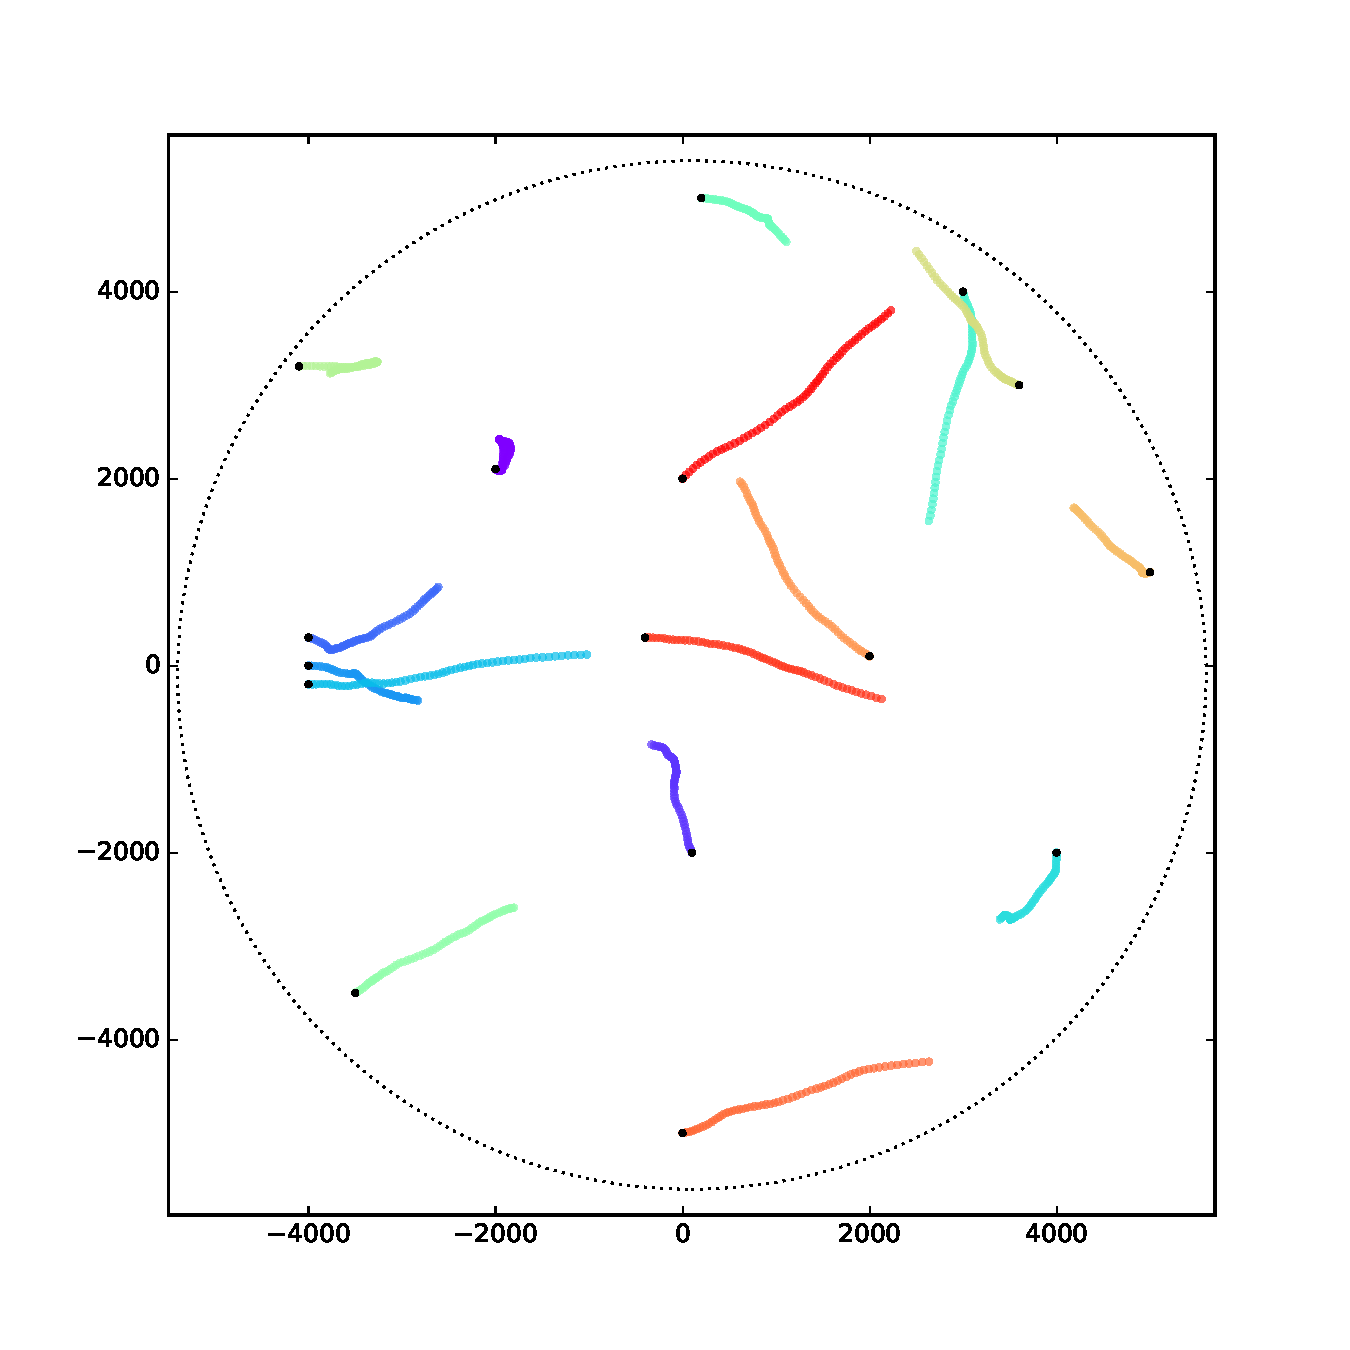
\includegraphics[width = .8\textwidth]{Figures/scenarioTruth.pdf}
\caption{True tracks}\label{fig:test_scenario}
\end{figure}
From these tracks, four scenarios where generated with different AIS configuration on the vessels, see Table~\ref{tab:ais_scenarios}
\begin{table}
\centering
	\begin{tabularx}{0.5\textwidth}{XXXXX}
	  \multicolumn{5}{c}{AIS scenario configuration} \\
	  \toprule
	  		 & \multicolumn{4}{c}{Scenario} \\
	  Target & 1 	& 2 	&  3 	&  4 	\\
	  \midrule
	  0 	& --- 	& B 	& --- 	& A 	\\
	  1 	& --- 	& B 	& --- 	& A 	\\
	  2 	& --- 	& B 	& --- 	& A 	\\
	  3 	& B 	& B 	& A 	& A 	\\
	  4 	& --- 	& B 	& --- 	& A 	\\
	  5 	& --- 	& B 	& --- 	& A 	\\
	  6 	& --- 	& B 	& --- 	& A 	\\
	  6 	& --- 	& B 	& --- 	& A 	\\
	  6 	& --- 	& B 	& --- 	& A 	\\
	  7 	& --- 	& B 	& --- 	& A 	\\
	  8 	& --- 	& B 	& --- 	& A 	\\
	  9 	& B 	& B 	& A 	& A 	\\
	  10 	& --- 	& B 	& --- 	& A 	\\
	  11 	& --- 	& B 	& --- 	& A 	\\
	  12 	& B 	& B 	& A 	& A 	\\
	  13 	& --- 	& B 	& --- 	& A 	\\
	  \bottomrule
	\end{tabularx}~\caption{AIS scenario configuration}\label{tab:ais_scenarios}
\end{table}